\documentclass[submitting]{nst}
\usepackage{subfigure,dcolumn}
\usepackage[T2A,T1]{fontenc}
\usepackage[english]{babel}

% The following package will be used to typeset the LaTeX codes and is not a necessity to this template
\usepackage{listings}
\lstloadlanguages{[LaTeX]TeX}
\lstset{language=[LaTeX]TeX,keywordstyle=\color{red},showspaces=true,breaklines=true,breakatwhitespace=true,basicstyle=\small\tt,commentstyle=\color{white},frame=single,framerule=0pt,backgroundcolor=\color{yellow}}


\begin{document}


\title{The MuTe simulation response to charged particles}

\author{A. Vásquez-Ramírez}
\email[Corresponding author:]{Carrera 27 calle 9 Ciudad Universitaria. Bucaramanga, Colombia., +57 3165084443, adrianacvr67@gmail.com}
\affiliation{Escuela de Física, Universidad Industrial de Santander, Bucaramanga Colombia}

\author{M. Suárez-Durán}
\affiliation{Departamento de F\'{\i}sica y Geolog\'{\i}a, Universidad de Pamplona, Pamplona-Colombia.}

\author{A. Jaimes-Motta}
\affiliation{Escuela de Física, Universidad Industrial de Santander, Bucaramanga Colombia}


\author{R. Calderón-Ardila}
\affiliation{Instituto de Tecnologías en Detección y Astropartículas, Centro Atómico Constituyentes,Comisión Nacional de Energía Atómica, Buenos Aires, Argentina}
\affiliation{Universidad Nacional de San Martín, Instituto SABATO, Argentina}

\author{J. Peña-Rodríguez}
\affiliation{Escuela de Física, Universidad Industrial de Santander, Bucaramanga Colombia}

\author{J.D. Sanabria-Gómez}
\affiliation{Escuela de Física, Universidad Industrial de Santander, Bucaramanga Colombia}

\author{D. Sierra-Porta}
\affiliation{Escuela de Física, Universidad Industrial de Santander, Bucaramanga Colombia}
\affiliation{Centro de Modelado Cient\'{\i}fico, Universidad del Zulia, 4001 Maracaibo-Venezuela}

\author{H. Asorey}
\affiliation{Instituto de Tecnologías en Detección y Astropartículas, Centro Atómico Constituyentes,Comisión Nacional de Energía Atómica, Buenos Aires, Argentina}
\affiliation{Laboratorio Detección de Partículas y Radiación,
Instituto Balseiro y Centro Atómico Bariloche,
Comisión Nacional de Energía Atómica, San Carlos de Bariloche, Argentina}
\affiliation{Sede Andina, Universidad Nacional de Río Negro, San Carlos de Bariloche, Argentina}

\author{L.A. Núñez}
\affiliation{Escuela de Física, Universidad Industrial de Santander, Bucaramanga Colombia}
\affiliation{ Departamento de Física, Universidad de Los Andes, Mérida, Venezuela}


\begin{abstract} 
This paper presents a detailed computational \textsl{Geant4} modeling of a hybrid Muon Telescope and the estimation of its response under a muon flux at $2650$\,m a.s.l at Cerro Machín Volcano-Colombia. 
 The instrument combines two detection techniques: a hodoscope with two planes of plastic scintillator bars, and a Water Cherenkov detector, located behind the rear scintillator panel, which acts as an absorbing element and as a third active coincidence detector. The model includes the materials, geometries, dimensions, and the photo-sensitive devices of the detectors. 
From the results obtained, in agreement with several experimental setups, we propose a muon detection trigger in terms of the energy deposited in each component of the instrument.
\end{abstract}

\keywords{keyword1, ... }

\maketitle
%%%%%%%%%%%%%%%%%%%
%%%% SECTION 1 %%%%
%%%%%%%%%%%%%%%%%%%
\section{Introduction}\label{sec:introduction}
The muography is an emerging technology based on measuring the attenuation of a muon flux that crosses geological and anthropic structures \cite{Kaiser2019}. Recently, we are witnessing several new successful academic and commercial applications such as detection of hidden materials in containers \cite{BlanpiedEtal2015}, archaeological building scanning \cite{MorishimaEtal2017, GomezEtal2016}, nuclear plant inspection \cite{FujiiEtal2013}, nuclear waste monitoring, underground cavities \cite{SaracinoEtal2017}, the overburden of railway tunnels \cite{ThompsonEtal2019} and volcanology (\cite{TanakaOlah2019} and references therein). In Colombia, more than a dozen active volcanoes, which represent significant risks to the nearby population \cite{Cortes2016, Agudelo2016, Munoz2017}, motivate research groups to explore this technique \cite{AsoreyEtal2017B, SierraPortaEtal2018, PenaRodriguezEtal2018, GuerreroEtal2019, ParraAvila2019, PenarodriguezEtal2019}.  

Atmospheric muons originate from the decay of charged pions and kaons produced through the interaction of cosmic rays (\textsl{CRs}) with the nuclei of the Earth's upper atmosphere. The energy of these particles comprises a broad spectrum, but only those muons with the highest energies ($\sim 100$\textsl{GeV}  ) can cross hundreds of meters of rock \cite{MarteauEtal2012}. Besides, they are the most abundant charged particles that reach the sea level due to their high penetrating power (they only lose around $2$\textsl{GeV}   when crossing the whole atmosphere) \cite{MarteauEtal2012}. Also, the muons are easily detectable by using different techniques based on ionization, excitation, and the Cerenkov effect \cite{MarteauEtal2012}. 

Hodoscopes are the most common detectors implemented for volcano muography.  They consist of two or several panels to identify the particle trajectories in terms of the zenith and azimuth angles. Projects like \textsl{MU-RAY} \cite{AnastasioEtal2013}, \textsl{ToMuVol} \cite{CarloganuEtal2013}, and \textsl{DIAPHANE} \cite{LesparreEtal2010} employ hodoscopes based on different detection technologies: emulsion plate, Resistive Plate Chambers, Micromegas, Multi-Wire Proportional Cameras, and scintillators, to mention the most common. Each of these techniques has advantages and disadvantages. The emulsion plate detectors \cite{MorishimaEtal2017, Nagamine2016} provide an excellent spatial resolution of the order of sub-microns, are passive, and easy to handle. On the other side, they have short lifetimes, and it is not possible to discriminate the time-stamp of dynamic phenomena, because the recorded events accumulate in the plates. The gas detectors as Resistive Plate Chambers \cite{SehgalEtal2016, Fehr2012}, Micromegas \cite{BouteilleEtal2016}, and Multi-Wire Proportional Cameras \cite{OlahEtal2018}, allow obtaining short traces of the detected particles with a spatial resolution around the microns. However, since these detectors operate outdoors, the gain of the electrodes depends highly on environmental variables such as pressure and temperature. Besides, they require high voltage for optimal operation, which results in higher power consumption compared with emulsion detectors. Finally, there are scintillator detectors such as the segmented \cite{FujiiEtal2013, LesparreEtal2012, TanakaEtal2009} and continuous \cite{NagamineEtal1995, AguiarEtal2015, TangEtal2016},  that are more robust since these do not have a high mechanical variation with environmental conditions, are easily constructed at a much lower cost than gaseous and emulsion detectors. Nevertheless, their spatial resolution is not as good as the other detectors since the segments generally used are of the order of centimeters.

This paper presents a detailed computational \textsl{Geant4} modeling of a hybrid Muon Telescope (\textsl{MuTe}) and the estimation of its response under a muon flux at $2650$\,m a.s.l at Cerro Machín Volcano-Colombia. The model includes the materials, geometries, dimensions, and the photo-sensitive devices of the detectors. In the next section, we briefly describe the rationale behind the \textsl{MuTe} design. Section \ref{sec:hodoscope-response} discussed the response from scintillator bar hodoscope to the impacting cosmic ray background. We emphasize in the bar scintillator model and the possible attenuation effects. In section \ref{sec:bar-data}, we compare our simulation results with data emerging from an experimental laboratory setup and study the temperature effect on breakdown voltage for the silicon photo-multiplier (\textsl{SiPM}). Section \ref{sec:wcd-response} presents the response of the Water Cerenkov Detector (\textsl{WCD}) and also compare some of the results with recent lab measurements. Finally in section \ref{sec:conclusions} we summarize some finals remarks and conclusions.

%%%%%%%%%%%%%%%%%%%
%%%% SECTION 1 %%%%
%%%%%%%%%%%%%%%%%%%

\section{The MuTe instrument design}
The Muon Telescope (sketched in figure \ref{fig:mute-detector}) is a hybrid detector that combines two technologies: a two-panel scintillator bar hodoscope, and a \textsl{WCD}, to filter most of the backward \& background noise \cite{NishiyamaMiyamotoNaganawa2014, KusagayaTanaka2015, NishiyamaEtal2016, GomezEtal2017}. This detector is capable of estimating not only the incoming  directions but also a range of energies of the impacting muons \cite{AsoreyEtal2017B, PenarodriguezEtal2019}.
  
 The panels of the hodoscope consist in an array of $30$ vertical $\times 30$ horizontal scintillator bars, of $4$cm wide, $2$cm high and $120$cm long, providing a resolution of $900$ pixels of $4$cm $\times 4$cm each one. This array yields a detection surface of $14.400$cm$^2$. 
 
 The \textsl{WCD} is a metal purified water container of $120$cm side, coated inside by the Tyvek with a photo-multiplier tube (\textsl{PMT}) on top to detect the Cerenkov photons (see figure \ref{fig:mute-detector}).

\begin{figure}
    \centering
    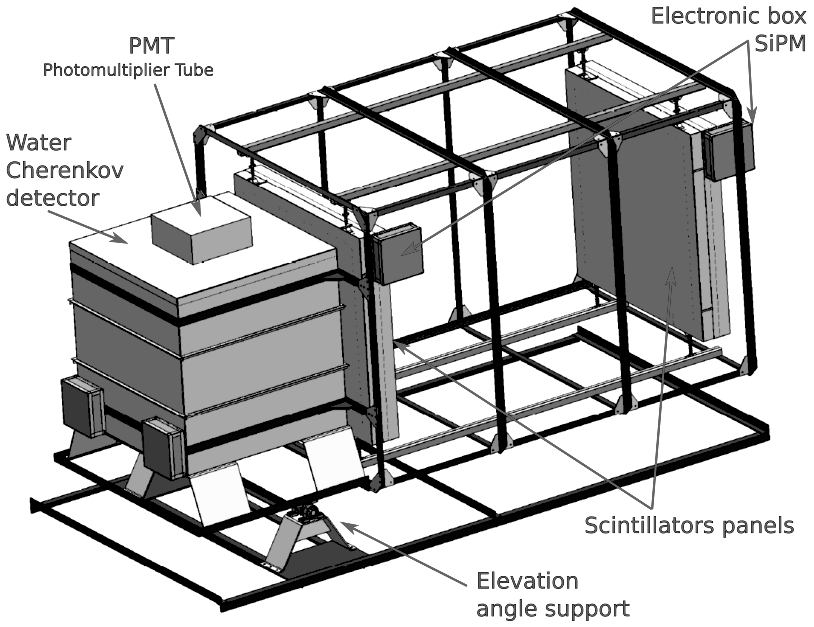
\includegraphics[scale=0.3]{Figures/mute-detector.png}
    \caption{The scketch of the hybrid detector \textsl{MuTe}: a two-panel scintillator bar hodoscope in front and a Water Cerenkov Detector at the back. Each panel of the scintillator bar hodoscope has $900$ pixels of detection to determine the incoming directions of the particles. The \textsl{WCD} is a metal purified water container of $120$cm side, coated inside by the Tyvek with a \textsl{PMT} on top to detect the Cerenkov photons. It is devised to filter most of the backward \& background noise of muography. The mechanical structure has a variable elevation angle to adjust the telescope according to the object under study.} 
    \label{fig:mute-detector}
\end{figure}

%%%%%%%%%%%%%%%%%%%
%%%% SECTION 2 %%%%
%%%%%%%%%%%%%%%%%%%
\section{Hodoscope response to cosmic ray background radiation}
\label{sec:hodoscope-response}
The response of the hodoscope bars refers to the signal produced in the photo-sensor when a minimum ionizing particle (\textsl{MIP}) crosses each scintillator bar. As shown in figure \ref{esquema_centelladora}, charged particles crossing the bars produce scintillation photons, absorbed, re-emitted, and guided to the photo-sensor device by a wavelength shifting (\textsl{WLS}) multi-cladding fiber. 

The bars of \textsl{MuTe} are Dow Styron $663$, made of Polystyrene, doped with $1$\% \textsl{PPO} and $0.03$\% \textsl{POPOP} \cite{PlaBrossRykalin2003}, which place a photon emission peak around the $420$nm wavelength. These bars, coated with $85$\% Polystyrene and $15$\% TiO$_2$ of $0.25$mm thick, have a tunnel of $\sim 3$mm diameter at its center, where there is a \textsl{WLS} multi-cladding fiber (reference BCF92 of Saint Gobain). The fiber diameter is $1$mm, with a core made of Polymethyl methacrylate, having the first clad of Polyethylene, and the second one of Fluorinated Polyethylene \cite{SaintGobain2017}. A mechanical coupling joins the fiber with a \textsl{SiPM} S$13360$-$1350$CS of Hamamatsu, with a photo-sensitive surface of $1.3$cm $\times 1.3$cm of $2668$ pixels \cite{Hamamatsu2018}. This device has a spectral detection range from $270$ to $900$nm, with its maximum sensitivity around $450$nm.

\begin{figure}[h!] %Rocal
    \centering
        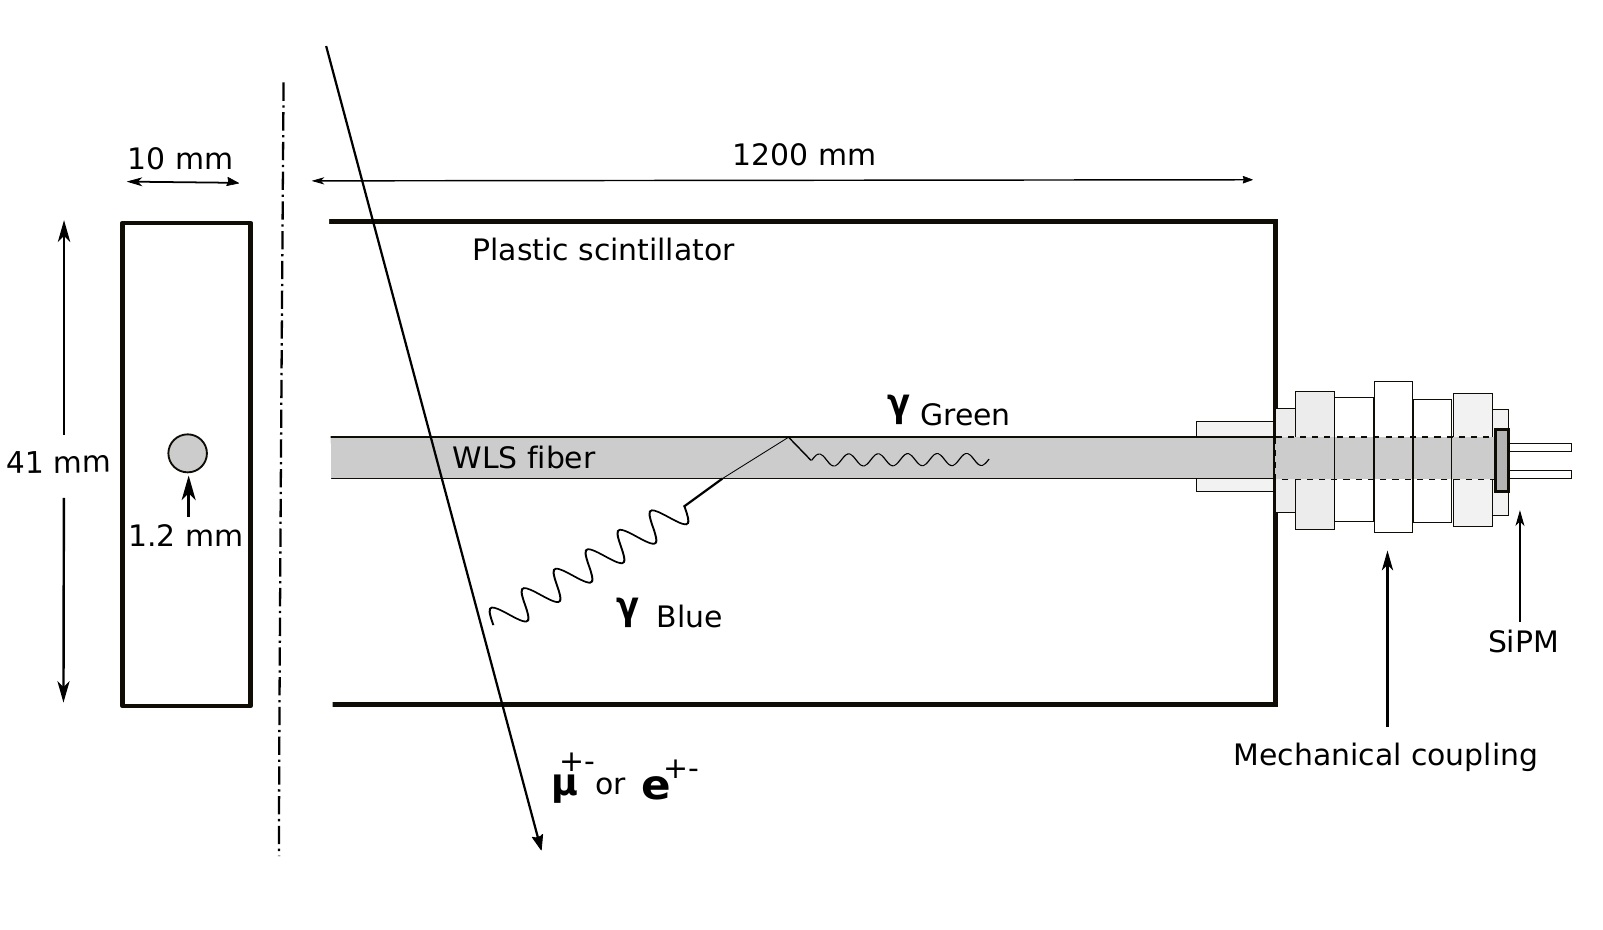
\includegraphics[scale=0.21]{Figures/esquema_barra.jpeg}
   \caption{This picture represent the scintillator bar system, with an embedded \textsl{WLS} fiber used for the experimental study of plastic scintillators coupled to a \textsl{SiPM}, what is remarkable, plastics are chosen to change the wavelength. When a charged particle cross the bar it losses part of its energy that generates photons with wavelength around the blue. Those photons are absorbed and re-emitted in the fiber as green photons. This fiber guides the photons to the \textsl{SiPM} where they produce a signal depending on their wavelength (its spectral detection range is $270$ to $900$nm with the maximum sensitivity around $450$nm).}\label{esquema_centelladora}
\end{figure}

Next sections will discuss the \textsl{Geant4} simulation model of the bars, as well as the experimental setup for the analysis of their responses (see section \ref{sec:bar-data}) and estimation of the average response of the hodoscope panels to the passage of \textsl{MIPs} (see section \ref{sec:hodoscope-response-two}). 


%%%%%%%%%%%%%%%%%%%%%%%%%%%
%%%%%%% SUBSECTION %%%%%%%%
%%%%%%%%%%%%%%%%%%%%%%%%%%%
\subsection{The scintillator bar model} \label{sec:bar-simulation}%Adriana
The scintillator bar \textsl{Geant4} geometric model is a parallelepiped of $4$cm wide, $2$cm high and $120$cm long. We incorporate to this geometry a coating material --made of $15$\% of TiO$_2$ and $85$\% of polystyrene-- with a reflectivity of $1$ and $0.25$mm of thickness.

The scintillating bar is polystyrene, with an index of refraction, $n=1.50$, and a photon absorption length of $5.5$cm. There is a tunnel of $119.5$cm long and $1.8$mm of diameter, drilled through the central axis of the bar, where we place a multi-cladding \textsl{WLS} fiber. This looseness of $0.5$cm at the end of the tunnel --filled with air to make the model as real as possible-- avoids the escape of photons.

A solid cylinder of poly-methyl methacrylate, with $119.45$cm long and $0.5$mm radius, models the fiber. This configuration leaves a space of $0.05$cm inside the tunnel to locate the \textsl{SiPM}. The first clad of this fiber is a cylindrical shell of polyethylene, with an internal radius of $0.5$mm and an external radius of $0.515$mm. The second is a shell of fluorinated polyethylene, with an internal radius of $0.515$mm and an external radius of $0.530$mm. Both coatings have the same fiber length.

A square surface of a side of $1.3$mm, attached to one of the fiber, represents the \textsl{SiPMs}. The simulations allow to set the \textsl{SiPM} photon detection efficiency, which depends on the wavelength, $\lambda$, of the photon hitting the \textsl{SiPM}, where the highest probability of photo-electrons (\textsl{pe}) generation is around $470$nm \cite{Hamamatsu2018}.

Figure \ref{fig:mips} displays the simulation results of the scintillator bar response to charged particles of different energy. The histogram of the number of photo-electrons generated by $10000$ electrons of $20$\textsl{MeV}, $100$\textsl{MeV} and $500$\textsl{MeV} has the same profile as those corresponding to the $10000$ muons of $1$\textsl{GeV}, $10$\textsl{GeV} and $100$\textsl{GeV}. This similarity occurs because both particles have the same stopping power in polystyrene, so they all deposit about $2.08$MeV of energy when passing through a centimeter of polystyrene (see equation \ref{energy_deposited}). Therefore, our detector is not able to distinguish muons from electrons, and it is necessary to use the \textsl{WCD} to select the muon events from noise. 

\begin{figure}
    \centering
    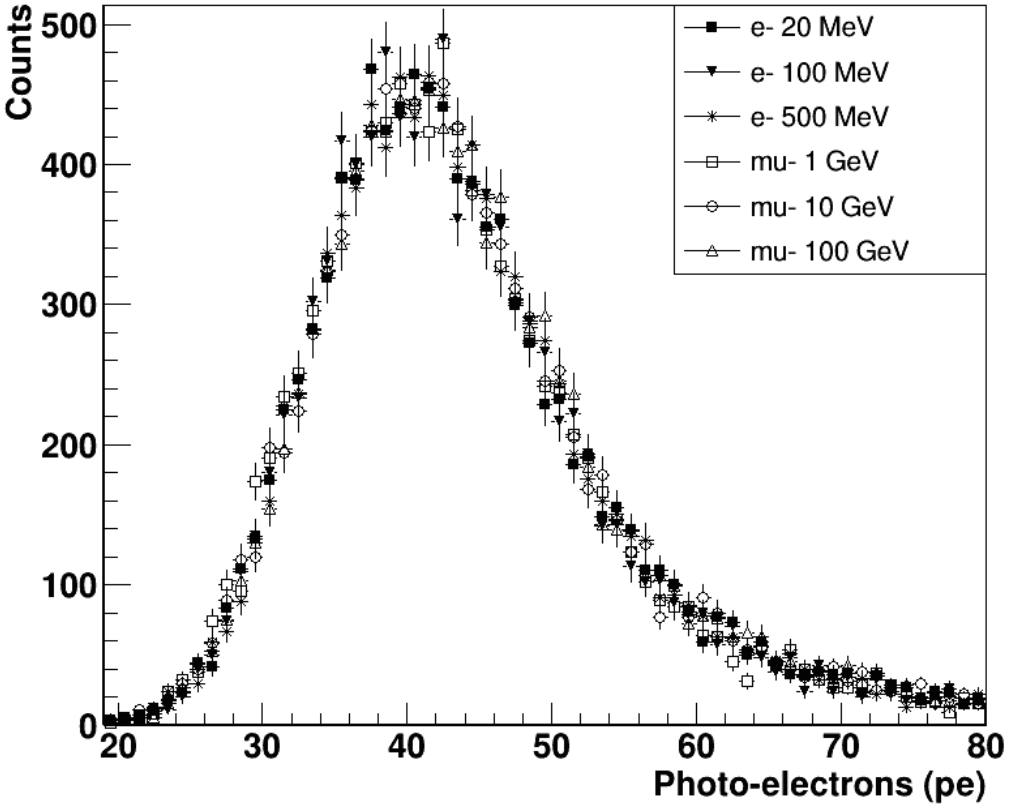
\includegraphics[scale=0.24]{Figures/MIPS.png}
    \caption{Scintillator bar response to \textsl{MIPs} of different energy. As expected, both electrons and muons generate the same histogram profile, since the energy loss of all those particles is $\sim 2.08$\textsl{MeV}. This result validates the code used and therefore supports the veracity of the simulations of the scintillator bar.
    To obtain those histograms, we performed the interaction of 10000 particles (of each energy and type) with the bar. The average number of photo-electrons is around $40$\textsl{pe} for all the particles, i.e., this detector is not able to distinguish muon events from noise.}
    \label{fig:mips}
\end{figure}

The mean value of those histograms is around $40$\textsl{pe}. For muons with energy of the order of \textsl{GeV}, the stopping power in the polystyrene is $\frac{dE}{d\varrho_\mathrm{pol}}\approx 2 \,\text{MeV cm}^2\text{/g}$ \cite{MichaelEtal2008}. Since those particles pass through the bar vertically, the distance traveled is $l_\mathrm{pol}=1$ cm. Hence, $40$\textsl{pe} is equivalent to $2.08$MeV of energy deposited in the bar ($E_\mathrm{d}$), according to equation \ref{energy_deposited}, where $\rho_\mathrm{pol}=1.04$ g/cm$^3$ is the polystyrene density. 

\begin{equation}
\label{energy_deposited}
\begin{split}
    E_\mathrm{d} &= 2 \,\text{  \textsl{MeV}  cm}^2\text{/g} \times \varrho_\mathrm{pol} \\
    &= 2 \,\text{  \textsl{MeV}  cm}^2\text{/g} \times l_\mathrm{pol} \times \rho_\mathrm{pol}\\
    &= \text{2.08} \, \text{  \textsl{MeV} }.
\end{split}
\end{equation}.

The following simulations are for muons with $3$\textsl{GeV} which are the most frequent at the level of our observation point on the Cerro Machín volcano. That is, from now on the \textsl{MIP} refers to this particle with this energy.

%%%%%%%%%%%%%%%%%%%%%%%%%%%
%%%%%%% SUBSUBSECTION %%%%%
%%%%%%%%%%%%%%%%%%%%%%%%%%%
\subsubsection{Attenuation of the photons in the \textsl{Bar}-\textsl{Fiber}-\textsl{SiPM} system}%Adriana
The light that propagates within the \textsl{WLS} fiber suffers an inevitable attenuation due to some photons escape from the optical guide, and others can be absorbed by the material while being transported to the \textsl{SiPM}. This attenuation depends on the length of the bar (which in this case is $120$cm), so it is necessary to study how the attenuation behaves in our \textsl{Bar}-\textsl{Fiber}-\textsl{SiPM} system. 

From the simulations of the scintillation detector, we can count the number of \textsl{pe} generated in the \textsl{SiPM} when a \textsl{MIP} crosses the bar at different distances $x$, where $x$ is the distance between the point of impact and the location of the \textsl{SiPM}. These distances were chosen to take into account the width of the pixels of the hodoscope, i.e., 4 cm wide; therefore $x$ varies as follows,
\begin{equation}
    x = (2+4p)\text{cm} \,\,\,\,\,\,\,\,\,\, p=0,1,2,...,29.
\end{equation}
Figure \ref{atenuacion_barra} shows the results of this simulation. If the particle impacts at the position closest to \textsl{SiPM} ($x=2$cm), it has the maximum photo-electron intensity and if it impacts  away form the \textsl{SiPM}, this intensity decreases. A double exponential function $F(x)$ fits the data and models this decrease
\begin{equation}
F(x)= \text{0.468}e^{-0.003(2-x)} + \text{0.531}e^{0.005(2-x)}.
\end{equation}
From this plot, we have that the attenuation in the \textsl{Bar}-\textsl{Fiber}-\textsl{SiPM} system is around $7$\%, that is agree with the experimental results, around $11\%$, given by figure \ref{experimental_attenuation}.
\begin{figure}[h!]
    \centering
        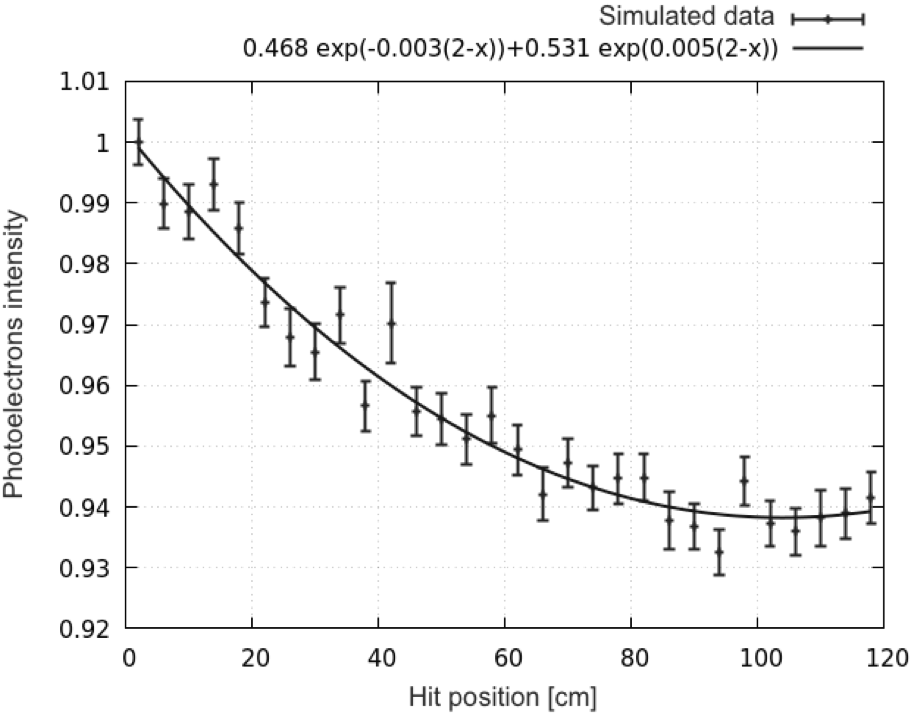
\includegraphics[scale=0.41]{Figures/atenuacion_barra_2.png}
   \caption{The number of photo-electrons concerning the position of the impacting \textsl{MIP} in the bar.    At $x=2$cm we have the maximum photo-electron intensity and as the particle impacts farther away to \textsl{SiPM}, the intensity decreases. A double exponential function fits the simulated data and this behavior can be associated with the attenuation of the photons traveling through the fiber, that is around $7$\%}
   \label{atenuacion_barra}
\end{figure}

The \textsl{MIP} detection with scintillator bar generates a number of \textsl{pe} in the \textsl{SiPM} at a time $t$. Now we want to estimate the time needed to collect the total number of photo-electrons produced. This total is about $40$\textsl{pe} at $x=2$cm, while at $x=118$cm it is about $37$\textsl{pe}. From the top of  figure \ref{cumulative} it can be noticed that $40$\% of the total photo-electrons occurred in the first $10$ns when the \textsl{MIP} has entered at $2$cm of the \textsl{SiPM}. Observe from the bottom of the figure \ref{cumulative} --when the \textsl{MIP} has entered at $118$cm of the \textsl{SiPM}--, that only 12\% of the \textsl{pe} is produced in the same time. In both cases, the total number of \textsl{pe} is reached around $80$ns, that is, the average time necessary to collect the total of \textsl{pe} produced by the passage of a muon, at any point of impact in the bar.
\begin{figure}[ht]
    \centering
    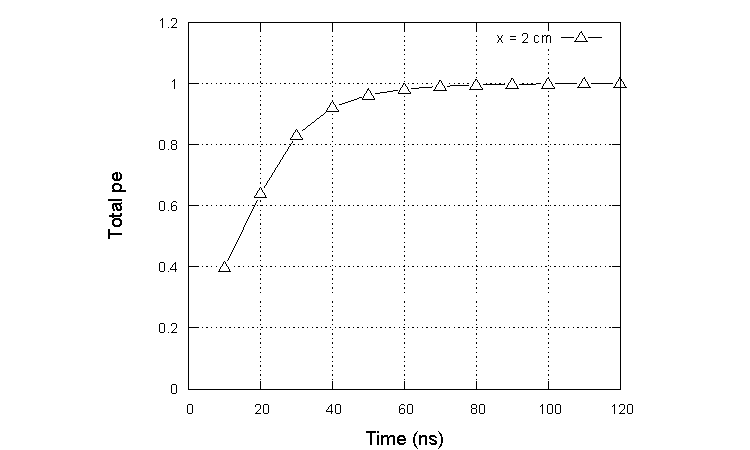
\includegraphics[scale=0.8]{Figures/cumulativo_1.pdf}
    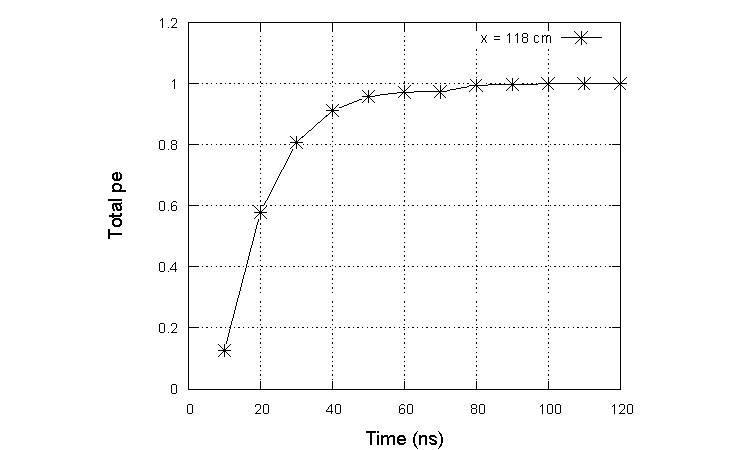
\includegraphics[scale=0.8]{Figures/cumulativo_2.pdf}
    \caption{Cumulative number of photo-electrons produced when a \textsl{MIP} hit the bar at $2$cm from the  \textsl{SiPM} (top) and at $118$cm (bottom). It can be noticed that $40$\% of the Total \textsl{pe} occurred in the first $10$ns when $x=2$cm and when $x=118$cm, only $12$\% of the \textsl{pe} is produced in the same time. In both cases, the total number of \textsl{pe} is reached around $80$ns, that is, the average time necessary to collect the total of \textsl{pe} produced by the passage of a muon, at any point of impact in the bar.}
    \label{cumulative}
\end{figure}

%%%%%%%%%%%%%%%%%%%%%%%%%%%
%%%%%%% SUBSUBSECTION %%%%%
%%%%%%%%%%%%%%%%%%%%%%%%%%%
\subsubsection{ \textsl{SiPM} and fiber coupling}%Adriana
The \textsl{Geant4} model allows estimating how good is the coupling \textsl{SiMP}-fiber. We define the ideal \textsl{SiMP}-fiber when they are side by side, without any space between them. Thus, all the traveling photons at the edge of the fiber impact directly on the \textsl{SiPM}. As shown above, the obtained average number of photo-electrons, for an ideal coupling, is $40$pe. A non-ideal coupling has space (filled with air) of $1.15$mm between the \textsl{SiPM} and the fiber. The number of \textsl{pe} is reduced to $8$, representing a loss of 80\% of the signal compared to the ideal case, as shown in figure \ref{coupling}.
\begin{figure}
    \centering
    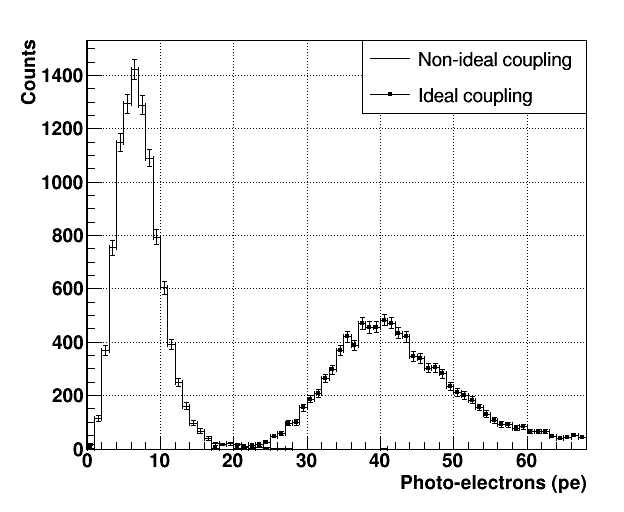
\includegraphics[scale=0.41]{Figures/coupling.png}
    \caption{Histogram of the number of \textsl{pe} resulting from the evaluation of the \textsl{SiPM} and fiber coupling. The squares curve represents the photo-electrons produced in the ideal case (when the \textsl{SiPM} and the fiber are side by side), while the simple line shows the non-ideal case, where the distance between the \textsl{SiPM} and the fiber is $1.15$mm. The average number  in the ideal case is around $40$\textsl{pe} and in the non-ideal is around $8$\textsl{pe}, i.e. the $80$\% of the signal is lost. This result gives an idea of when a bar-fiber-\textsl{SiPM} system of the real detector is badly coupled and should be replaced or verified.}
    \label{coupling}
\end{figure}


%%%%%%%%%%%%%%%%%%%%%%%%%%%
%%%%%%% SUBSECTION %%%%%%%%
%%%%%%%%%%%%%%%%%%%%%%%%%%%
\subsection{Experimental results from the scintillator detector}
\label{sec:bar-data}%Rolando
The plastic scintillators of the \textsl{MuTe} panels are active detectors that work as counters of charged particles. This allows the indirect detection of ionizing radiation, due to the light --produced in the scintillator at the passage of a charged particle-- travels through the optical fiber towards the \textsl{SiPM}, where it produces an electrical signal which can be analyzed offline. The diagram of this \textsl{Bar}-\textsl{Fiber}-\textsl{SiPM} system is represented in figure \ref{esquema_centelladora}. 

Since the \textsl{SiPMs} have intrinsic noise,  it is essential to know well the detector to define a methodology with a discriminant to detect particles and correctly interpret the measured data. A first study was made to guarantee that the \textsl{SiPM} keeps working in Geiger mode at any temperature. Section \ref{breakdown-voltage} presents the results of the dependence of the breakdown voltage with the temperature.

On the other hand, given that the scintillator, the fiber, and the \textsl{SiPM} are not $100$\% efficient, there are various parameters to take into account. For example, the material of the bars is opaque to photons with an average length of $5.5$cm of attenuation. Then, to have a detector of $120$cm length, a \textsl{WLS} fiber is placed inside the bar. The fibers guide the photons, but they can experiment attenuation despite being multi-layer, i.e., some photons can escape from the guide and even reflected in the border. This represents an additional problem when coupling different scintillators, and there will be edge effects related to the refractive index of each one. Therefore, we must quantify the attenuation in these fibers and determine whether the coupling and the attenuation will be relevant in the case of the MuTe scintillator bars. A controlled experiment was performed to estimate the percentage of attenuation in the system (see section \ref{attenuation-experimental}).

%%%%%%%%%%%%%%%%%%%%%%%%%%%
%%%%%%% SUBSECTION %%%%%%%%
%%%%%%%%%%%%%%%%%%%%%%%%%%%
\subsubsection{Dependence of the breakdown voltage with the temperature}
\label{breakdown-voltage}
To study the response of each scintillator bar, we first studied the \textsl{SiPMs} thermal stability. \textsl{SiPMs} can change their mode of operation if the input voltage ($V_{Bias}$) is less than the breakdown voltage ($V_B$), and this parameter varies with temperature. Thus we need to find this functionality to guarantee that \textsl{SiPMs} always works in Geiger mode 

To establish this dependence, we build a temperature-controlled box regulated by a TEC1-12706 thermoelectric Peltier, mounted on an aluminum frame, where we place the mechanical coupling of the \textsl{SiPM}.  The control system consists of two sensors: one to vary the temperature and the other one to measure it on the \textsl{SiPM}. Figure \ref{timesetup} displays the results for the operation of this system for different target temperatures ($10^{\circ}$C, $20^{\circ}$C, $40^{\circ}$C and $50^{\circ}$C).  Note that the time required to reach the target temperature, in each case, is around $(600 \pm 50)$s.
\begin{figure}[h!] 
    \centering
        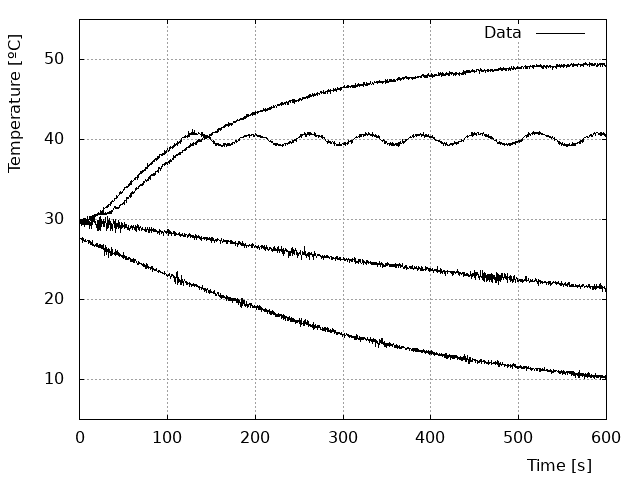
\includegraphics[scale=0.48]{Figures/tiempo_establecemiento.png}
   \caption{Measurements of the system set-up time with different target temperatures: $10^{\circ}$C, $20^{\circ}$C, $40^{\circ}$C and $50^{\circ}$C. We can see that the time required to reach the target temperature in each case is around $(600 \pm 50)$s. }
   \label{timesetup}
\end{figure}

Next, Dark-Current \cite{Renker2006} measurements follow in the range for $40$V to $60$V, for different temperatures and figure \ref{temperature} illustrates the linear temperature dependence of  $V_B$. It is clear that  for each $10^{\circ}$C of temperature, the $V_B$ changes around $0.45$V.
\begin{figure}[h!] %Rocal
    \centering
        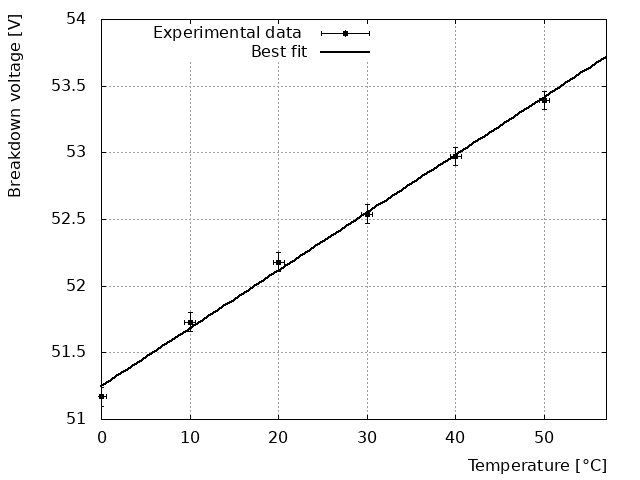
\includegraphics[scale=0.49]{Figures/voltajeRuptura.png}
   \caption{Dependence of the breakdown voltage with the temperature for the \textsl{SiPM} Hamamatsu S13360-1350CS used in the MuTe hodoscope. It can be observed that the relation is linear, that is for every $10^{\circ}$C of temperature the $V_B$ varies about $0.45$V.}\label{temperature}
\end{figure}

%%%%%%%%%%%%%%%%%%%%%%%%%%%
%%%%%%% SUBSECTION %%%%%%%%
%%%%%%%%%%%%%%%%%%%%%%%%%%%
\subsubsection{Attenuation measurements of the \textsl{Bar}-\textsl{Fiber}-\textsl{SiPM} system}\label{attenuation-experimental}%Rolando
To estimate the attenuation in the scintillator bars, we measure the signal produced by the passage of charged particles at both ends and the middle of the bar. Figure \ref{coincidencia_barras} illustrates the experimental set-up, which defines an event if there is a simultaneous signal in the three scintillators: the upper, the bar, and the lower one. 

\begin{figure}[h!] %Rocal
    \centering
        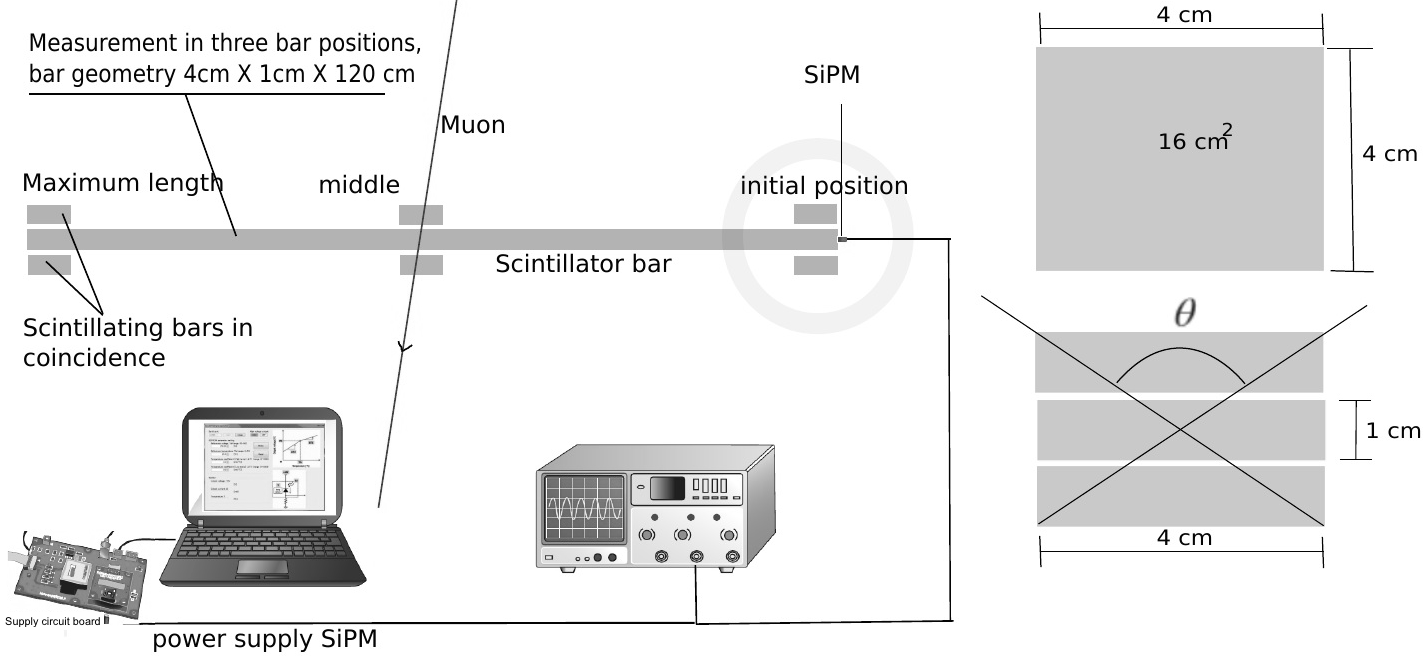
\includegraphics[scale=0.23]{Figures/barras_coincidencia.png}
   \caption{Diagram of the experimental set-up to measure the bar signal attenuation. The three positions of interest are at both ends and the middle. An event is if there is a simultaneous signal in the three scintillators: the upper, the bar, and the lower one.} 
   \label{coincidencia_barras}
\end{figure}

The trigger system, connected to a RedPitaya development card, records pulses with a frequency of 125 Mhz \cite{Pitaya2016}. The system was synchronized to have pulses in coincidence, producing three input signals to the card and one output signal that corresponds to each position in the scintillator test bar. The coincidence system has an angle $\theta$ for this configuration of $106.26^{\circ}$, as shown in figure \ref{coincidencia_barras}. The frequency of events per minute, measured with an oscilloscope, was $10\pm1$ per minute for $16$cm$^2$. Thus, with this rate, it is possible to detect 0.62 particles$\times$min$\times$cm$^2$. 

After a noise calibration, we record $10000$ reference pulses in the three positions of interest. At the farthest end from the \textsl{SiPM}, the fiber was cut to $45^{\circ}$ to maximize photon leakage and to avoid secondary pulses by reflections at the end of the fiber. 

From each average pulse, we calculate the mean deposited charge at the three positions. Then, we estimate the percentage of attenuation by normalizing and comparing the values, as shown in figure \ref{experimental_attenuation}. In our case, the difference between the mean charge value deposited at both ends is around $11$\%.  There, an exponential adjustment coincides with the attenuated signal an the fitting function was 
$f(x)~=~0.88~+a*exp(-x*b)$ with the parameters $a=0.126652$, $b= 0.0205653$ with an error of  $\pm 0.003444 (2.72\%)$ and $\pm 0.001065 (5.18\%)$, respectively.
\begin{figure}[h!] %Rocal
    \centering
        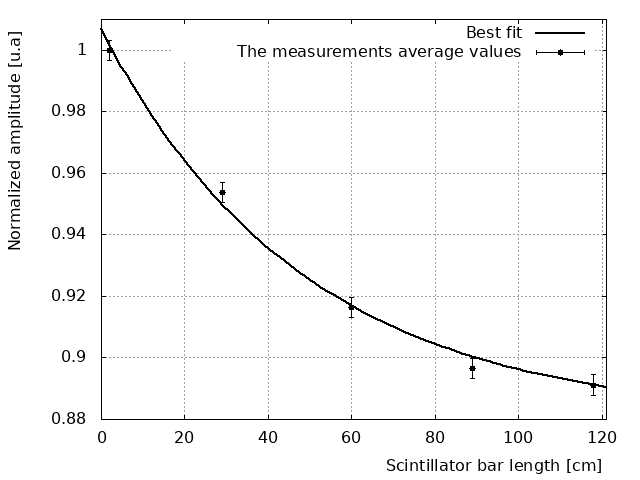
\includegraphics[scale=0.49]{Figures/atenuacion_esperimental.png}
   \caption{Attenuation of the signal in the test bar obtained from the coincidence of three signals. The maximum amplitude is in the position closest to the \textsl{SiPM}, decreases by 11\% at the opposite end.} \label{experimental_attenuation}
\end{figure}

%%%%%%%%%%%%%%%%%%%%%%%%%%%
%%%%%%% SUBSECTION %%%%%%%%
\subsection{Simulated attenuation in the hodoscope}
\label{sec:hodoscope-response-two} %Adriana
The probability of producing photo-electrons in the \textsl{SiPM} of horizontal and vertical bars is a crucial concept to determine the response of each panel of the hodoscope. The bar simulation generates the response of a detection panel to \textsl{MIPs} . Thus, independent events in a particular pixel $P^{F}_{i,j}$ is given by 
\begin{equation}
\label{pe_panel}
P^{F}_{i,j}=P^{F}_{i} \times P^{F}_{j},
\end{equation}
where $P^{F}_{i}$ y $P^{F}_j$ are the probabilities obtained in the horizontal bar $i$ and in the vertical bar $j$, respectively.

Figure \ref{atenuacion_panel_bw} displays the probability of photo-electrons produced by \textsl{MIPs} and hitting each panel pixel, obtained from equation \ref{pe_panel}.
\begin{figure}[h!]
    \centering
        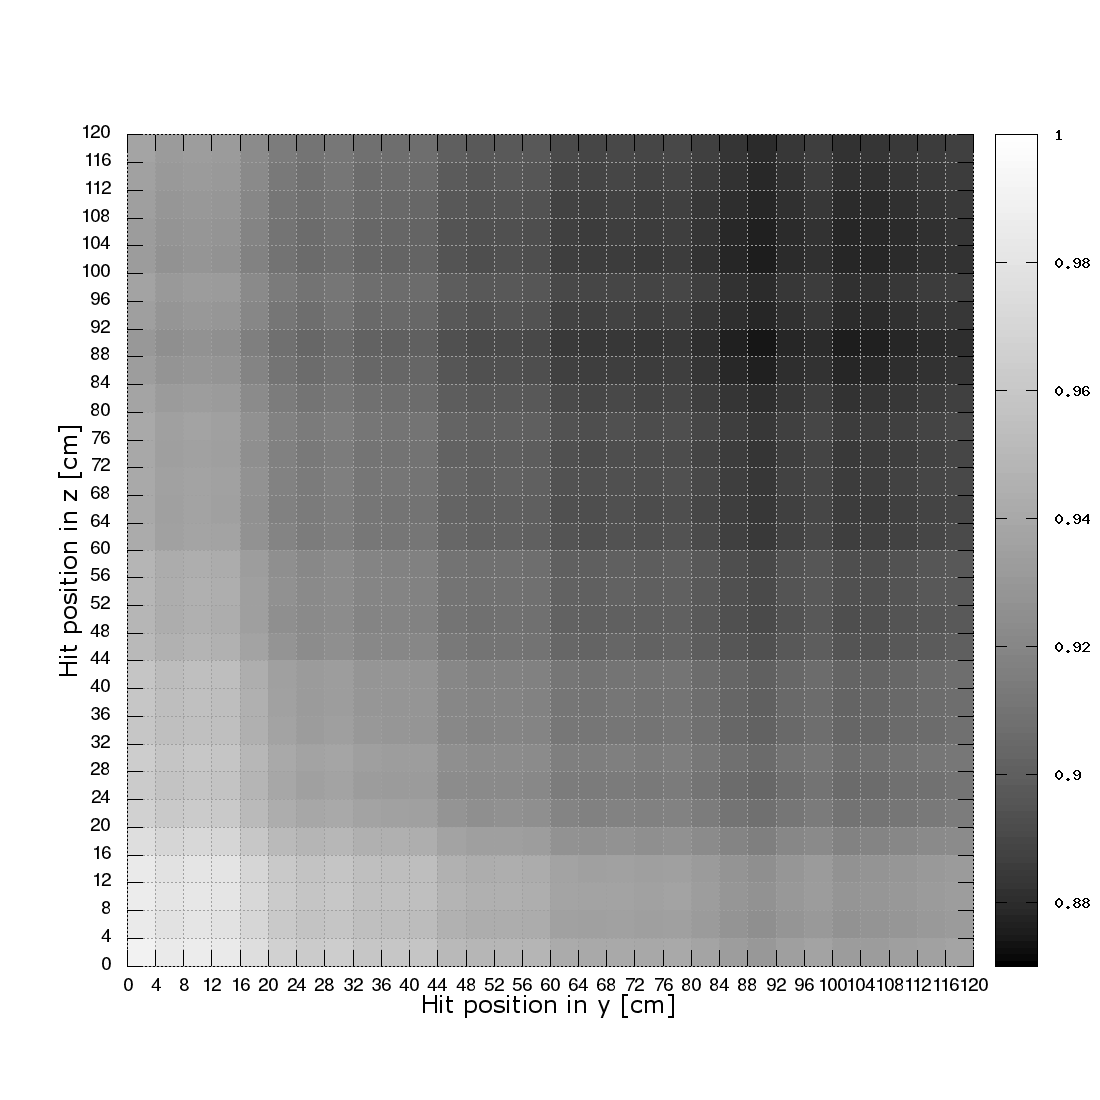
\includegraphics[scale=0.3]{Figures/atenuacion_panel_bw.png}
   \caption[Response of the hodoscope panels]{Production probability of photo-electrons in each of the pixels of a panel of the hodoscope by muons of 3   \textsl{GeV}  of energy. Each frame represents a detection pixel and it can be seen that there is a difference between two zones of the panel. In the pixel $P_{11}$, where the \textsl{SiPM} of the horizontal bar and the vertical bar is only 2 cm from the point of impact of the muon, is produced the maximum number of \textsl{pe} while the \textsl{pe} decreases until 12\% for pixels far from the SiPMs. This result is valid both for the front and the rear panel.}\label{atenuacion_panel_bw}
\end{figure}

These results are valid for both the front panel and the rear panel, and from figure \ref{atenuacion_panel_bw}, it clear that there is a difference between the zones. This difference around $12$\% can be associated with the attenuation of photons in the fiber, i.e., the pixels that are closer to the \textsl{SiPM} count more photo-electrons.  


%%%%%%%%%%%%%%%%%%%
%%%% SECTION 4 %%%%
%%%%%%%%%%%%%%%%%%%
\section{The water Cerenkov detector response to cosmic background radiation}
\label{sec:wcd-response}
The \textsl{WCD} indirectly detects charged particles, detecting the Cerenkov photons generated by particles traveling through the contained water. The photo-multiplier tube counts photo-electrons according to its quantum efficiency, which depends on the wavelength of the impacting photon.  In our case, the \textsl{PMT} Hamamatsu R5912 of the \textsl{MuTe} has a maximum detection probability value of $25$\% for photons with $\lambda = 400$ nm \cite{Hamamatsu2018}. The \textsl{PMT} located at the top of the metal container of purified water with $120$\,cm side, coated with a diffusive lining of Tyvek 

The following sections will discuss some of the results from the detector simulation, as well as the first data recorded by the  \textsl{WCD}.

%%%%%%%%%%%%%%%%%%%%%%%%%%%
%%%%%%% SUBSECTION %%%%%%%%
%%%%%%%%%%%%%%%%%%%%%%%%%%%
\subsection{The WCD model}\label{sec:wcd-model}
 In \textsl{Geant4} the water container is a stainless steel cube of length $l_c=1.21$m, with water inside water in a cube of $ l=1.20$m side. The water has a refractive index $n$, which varies between $1.3435$ and $1.3608$, and a photon absorption length ranging from $0.69$m to $2.90$m according to its energy. In the walls of the cube, the Tyvek is modeled as an optical surface with a reflection index $n_{\mathrm{Tyvek}} = 1 $, which diffuses the Cerenkov photons.

For the \textsl{PMT}, the photo-cathode was simulated as an air half-ellipsoid with semiaxes $s_x=10.1$cm, $ s_y = 10.1$cm and $s_z=6.5$cm, located on top of the water cube. The quantum efficiency (\textsl{QE}) of this device was introduced in the code, taking into account reference Hamamatsu R5912 \cite{Hamamatsu2018}. The QE determines whether photons reaching the outer surface of the photo-cathode will be detected or not. These photons originate photo-electrons (denoted as \textsl{pe}) by photoelectric effect. The \textsl{WCD} response  is given in terms of \textsl{pe} generated by each particle interacting with it.

Notice that the inclusion of the \textsl{QE} of the \textsl{PMT} in the code, as a function dependent on $\lambda$, represents an improvement over the simulations of \textsl{WCDs} carried out previously within the research group. An unique efficiency of $25$\% is taken into account in \cite{CalderonAsoreyNunez2015}, for the wavelength range between $330$nm and $570$nm. Therefore, the new code offers more precise results of the pulses produced by the passage of particles in water. 
 
 \begin{figure}
    \centering
    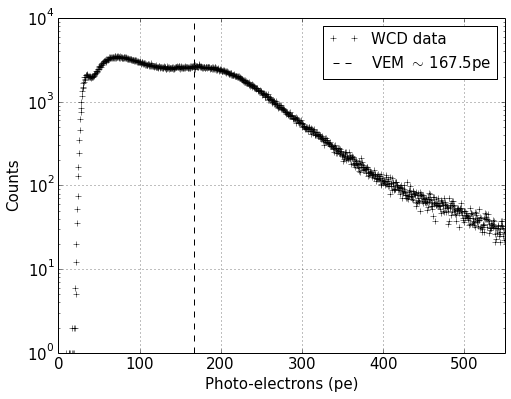
\includegraphics[scale=0.45]{Figures/WCDpedata.png}
    \caption{Photo-electron histogram for one hour of data recorded by the \textsl{WCD}. }
    \label{WCDpe}
\end{figure}

 
%%%%%%%%%%%%%%%%%%%%%%%%%%%
%%%%%%% SUBSECTION %%%%%%%%
 \subsubsection{Estimation of the Vertical Equivalent Muon unit}
The Vertical Equivalent Muon (\textsl{VEM}) --defined as the average charge collected in the \textsl{PMT} when a high-energy muon vertically crosses the entire detector --  is generally adopted as the unit to calibrate the energy deposited by incident particles and is independent of the detection position.   Muons can be easily identified by installing plastic scintillators above and below the \textsl{WCD} \cite{EtchegoyenEtal2005}.
 
\textsl{Geant4} code allows the injection of muons with a chosen energy and direction. We model injecting  $100000$ vertical muons with $3$\textsl{GeV}  in direction $-\hat{z}$ towards the water, and the initial position given by the point $ P=(80, 80, 121)$ cm, over the \textsl{WCD}. The portion of the number of Cherenkov photons, $N$, that reaches the external surface of the photo-cathode, is $N_{\mathrm{PMT}}$. 

 The $ N_{\mathrm{PMT}}$,  depending on its wavelength, produces a number of photo-electrons, $N_{\mathrm{pe}}$. We have estimated the efficiency of the \textsl{WCD} with the following chain of events. One \textsl{VEM} of $3$\textsl{GeV} generates around $46857$ Cherenkov photons in $120$cm. Next, only $1617$ of those photons reach the external surface of the photo-cathode, and, due to its quantum efficiency, around an average $203.2$ \textsl{pe} was produced. Thus, the system has a muon detection efficiency of $0.4$\%, that is,
\begin{equation}
\eta_{\mathrm{WCD}}=\frac{N_{\mathrm{FE}}}{N} 100\%=\frac{203.2}{46857}100\%=0\textnormal{.}4\%
\end{equation}

Figure \ref{WCDpe} displays the comparison of  the \textsl{VEM} simulated value ($\sim 203.2$ pe) with the measured  $\sim 167.5$pe. This figure represents the \textsl{pe} histogram for one hour of data for a discrimination threshold of $110$mV. The histogram has two prominent humps, the electromagnetic (electrons, positrons and gammas) hump at $\sim 70$\textsl{pe} and the muonic hump at $\sim 167.5$pe \cite{PenarodriguezEtal2019}.  

To compare the \textsl{WCD} response to muons and electrons  at the Cerro Machín Volcano, we run simulations for $100000$ vertical electrons, \textsl{VE}, of $20$\textsl{MeV} at the same initial direction and point $P$. Figure \ref{vem_ve} presents the corresponding histogram of the number of photo-electrons. The mean value of the \textsl{VE} is smaller than the \textsl{VEM}, around $16.7$\textsl{pe} that represents a $8$\% of it.

Next, in the number of \textsl{pe} vs time displayed in plot \ref{pulse_vem_ve} we sketch  the \textsl{VEM} and \textsl{VE} pulses. From those histogram fits, we can obtain the attenuation time $\tau$ and signal length $l_a$.  Finally, the table \ref{t:comparacion} sumarize the comparison between both charged particles.
\begin{figure}
    \centering
    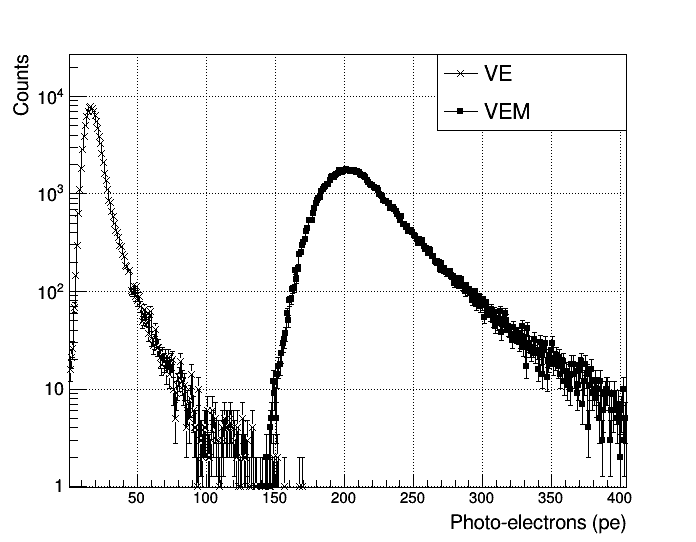
\includegraphics[scale=0.38]{Figures/vem_ve.png}
    \caption{Histogram of the number of photo-electrons produced due the detection of vertical muons (squares) and vertical electrons (crosses) with the \textsl{WCD}. From the squares curve, the mean value for the unit of calibration, \textsl{VEM}, is around $203.2$\textsl{pe}. In comparison, the mean number produced by the \textsl{VE} is $16.7$\textsl{pe}, that is the $8$\% of the \textsl{VE}. This results shows that the \textsl{WCD} }
    \label{vem_ve}
\end{figure}

\begin{figure}
    \centering
    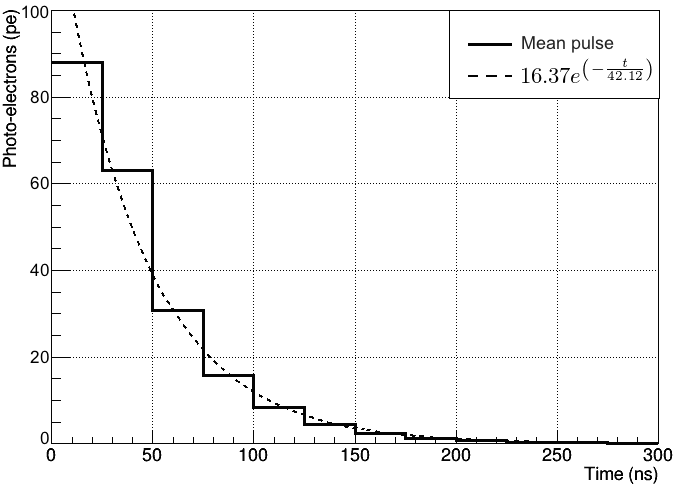
\includegraphics[scale=0.35]{Figures/pulse_vem.png}
    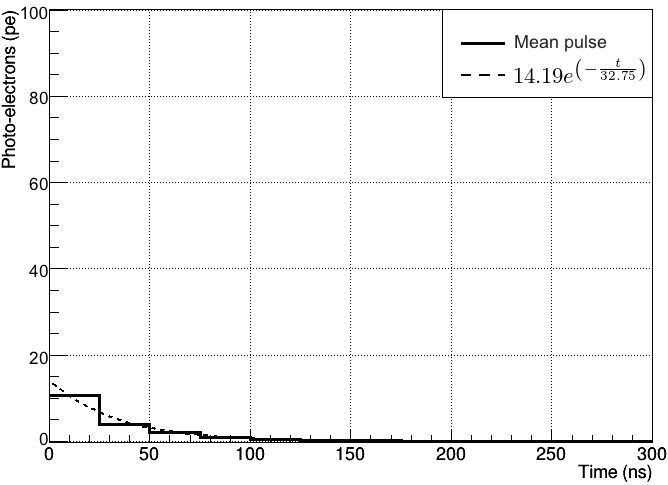
\includegraphics[scale=0.35]{Figures/pulse_ve.png}
    \caption{Mean pulse corresponding to the \textsl{VEM} (top) and the \textsl{VE} (bottom) response. The dashed lines represent the best exponential fit of the pulses where the attenuation time $\tau$ is around $42.12$ns for the \textsl{VEM} and $32.75$ns for the \textsl{VE}.}
    \label{pulse_vem_ve}
\end{figure}

\begin{table}[h!]
\label{t:comparacion}
\centering
\caption{Summary of the physical magnitudes obtained for the \textsl{VEM} and the \textsl{VE}: Length traveled in water ($l$), Number of Cherenkov Photons produced ($N$), Number of Photons that reach the \textsl{PMT} ($N_{\mathrm{PMT}}$), Number of Photoelectrons ($N_{\mathrm{FE}}$), Time of attenuation of the pulse ($\tau $) and Length of attenuation ($l_a$).}

\begin{tabular}{l|c|c|}
\cline{2-3}
                                                     & \textbf{$\mu^-$ (3   \textsl{GeV} ) }& \textbf{$e^-$ (20   \textsl{MeV} )} \\ \hline
\multicolumn{1}{|l|}{\textbf{$l$}}   &          (120 $\pm$ 1) cm      &    (10 $\pm$ 1) cm        \\ \hline
\multicolumn{1}{|l|}{\textbf{$N$}}    &         46857 $\pm$ 13 $ $   &      3538 $\pm$ 1 $ $      \\ \hline
\multicolumn{1}{|l|}{$N_{\mathrm{PMT}}$}       &          1617 $\pm$ 1     &     132.1 $\pm$ 0.1      \\ \hline
\multicolumn{1}{|l|}{$N_{\mathrm{pe}}$}       &          203.2 $\pm$ 0.2      &     16.729 $\pm$ 0.003       \\ \hline
\multicolumn{1}{|l|}{$\tau$} &          (42.12 $\pm$ 0.01) ns      &      (32.75 $\pm$ 0.03) ns      \\ \hline
\multicolumn{1}{|l|}{$l_a$} &          (7.332 $\pm$ 0.001) m      &      (9.430 $\pm$ 0.002) m      \\ \hline
\end{tabular}
\end{table}

%%%%%%%%%%%%%%%%%%%%%%%%%%%
%%%%%%% SUBSECTION %%%%%%%%
%%%%%%%%%%%%%%%%%%%%%%%%%%%
\subsubsection{WCD response to the cosmic ray background radiation}%Adriana
The \textsl{LAGO} \textsl{ARTI} framework allows us to estimate of the \textsl{WCD} response to the cosmic ray background radiation flux ($\Xi$) at any site \cite{SarmientoEtal2019}. This toolkit employs a \textsl{Geant4} code to estimate the number of Cerenkov photons detected by the \textsl{PMT} and employing its quantum efficiency. The \textsl{ARTI} framework uses the energy and the momentum of the particles from $\Xi$ as input and obtains the flux by using the \textsl{CORSIKA} code \cite{HeckEtal1998}, with a geomagnetic correction form \textsl{MAGCOS} code \cite{Desorgher2003}. For other examples of the precise simulation chain see  \cite{AsoreyEtal2015B, AsoreyNunezSuarez2018}. 

Figure \ref{fig:flux} plots the histogram of the number of photo-electrons, produced at Cerro Machín. The flux $\Xi_{CM}$, 
\begin{equation}
\Xi_{CM} = \frac{N_{\mathrm{Sec}}}{7.5\,\mathrm{s}\, 480\,\mathrm{m}^2}, 
\end{equation}
is calculated over a circular area $A=480$m$^2$ placed $1$cm above the detector, with a zenithal aperture of $0\leq \theta \leq 80^{\circ}$, and where $N_{\mathrm{Sec}}=$ represents the number of secondaries at this particular site.

 The different curves represent the contribution of various particles to the total response (empty circles). Note that this curve has two main peaks, the first one with a contribution of the electromagnetic component and the second one with the muonic component.
\begin{figure}
    \centering
    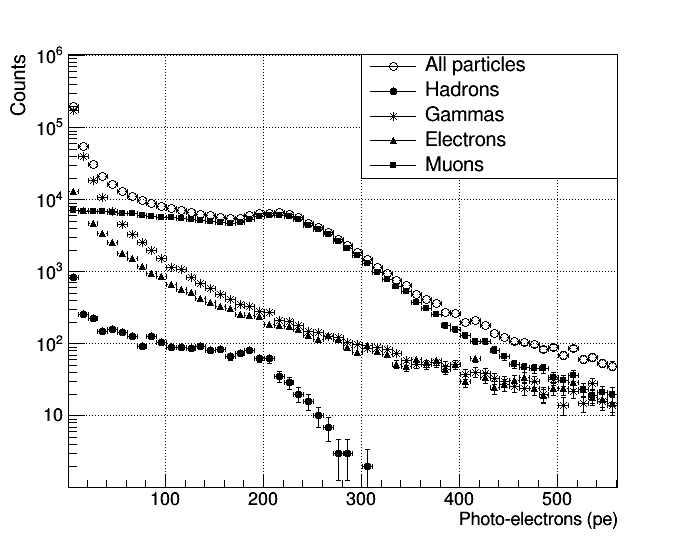
\includegraphics[scale=0.4]{Figures/flux.png}
    \caption{Histogram of the number of photo-electrons produced by all the particles, hadrons, gammas, electrons and muons detected in the \textsl{WCD}.}
    \label{fig:flux}
\end{figure}


%%%%%%%%%%%%%%%%%%%
%%%% SECTION 6 %%%%
%%%%%%%%%%%%%%%%%%%
\section{Conclusions}
\label{sec:conclusions}%Todos
As we have stated above, MuTe combines two detection techniques: a hodoscope with two detection planes of plastic scintillator bars, and a \textsl{WCD}, in an innovative setup which differentiates it from some previous detectors. 
\begin{itemize}
    \item \textbf{Scintillators panels:} Inspired by the experiences of other volcano muography experiments \cite{UchidaTanakaTanaka2009,GibertEtal2010}, we have designed two X-Y  arrays of $30 \times 30$ plastic scintillating strips ($120$cm$\times 4$cm$\times 1$cm), made with Styron$^{\textrm{TM}}$ 665-W polystyrene doped with a mixture of liquid organic scintillators: 1\% of 2,5-diphenyloxazole (PPO) and 0.03\% of 1,4-bis (5-phenyloxazol-2-yl) benzene (POPOP). Each array has $900$ pixels of $4$ cm$\times 4$ cm = $16$ cm$^2$, which sums up $14,400$ cm$^2$ of detection surface which can be separated up to $D=250$ cm.
    \item \textbf{Water Cherenkov Detector:} The \textsl{WCD} is a purified water cube of $120$\, cm side, located behind the rear scintillator panel, which acts as an absorbing element and as a third active coincidence detector. Due to its dimensions and location, it filters most of the background noise (low energies electrons, protons, and muons moving backward) which could cause overestimation in the hodoscope counts \cite{NishiyamaEtal2016}, and it is capable of isolating the muonic component of the incident particle flux.  From the charge histogram, obtained by time integration of the individual pulses measured in the WCD, it is possible to separate two components of the incident flux: electromagnetic part (photon, electron \& positron) and the $\mu-$component \cite{AsoreyEtal2015B}.
\end{itemize}

The Colombian MuTe combines particle identification techniques to discriminate noise background from data. It filters the primary noise sources for muography, i.e., the soft-component ($e^{\pm}$) of Extensive Air Showers (EAS) and scattered/upward-coming muons. Particle deposited energy identifies Electrons/positrons events in the WCD, while scattered and backward muons are rejected using a pico-second Time-of-Flight system.

From the \textsl{Geant4} modeling for the scintillator detector, we obtained that the number of \textsl{pe} decreases around $7$\% with respect to those produced at the end near of the \textsl{SiPM}. This reduction occurs due to the attenuation of the photons that travel in the fiber, since, the more distance they travel within it, the more energy they lose and lesser photons reach the \textsl{SiPM}s. This result is in agreement with the $11$\% attenuation obtained with the experimental setup described in section \ref{sec:bar-data}. This attenuation seems to be insignificant in the bar, but it is more noticeable in the hodoscope panels, since, the difference between the closest corner to the \textsl{SiPMs} and the furthest, is around $12$\%.

Regarding the \textsl{WCD} response, the value of the \textsl{VEM} obtained with the simulations and that obtained in the laboratory measurements, are in the same order of magnitude, but present a percentage difference of $18$\% with respect to the simulated value. This difference can be related by the various components of the electronics, where part of the signal can be lost.

From the results obtained, a muon detection trigger for the \textsl{MuTe} is proposed in terms of the energy deposited in each of its components. That is, the muon must deposit around $2.08$\textsl{MeV} in two scintillator bars on the front panel, then the same energy in two bars on the rear panel of the hodoscope, to finally discriminate the signal from the noise in the \textsl{WCD}. Then, the muon must deposit around 240   \textsl{MeV}  of energy in the \textsl{WCD} to be counted as an event.


\section*{Acknowledgments}
The authors acknowledge the financial support of  Departamento Administrativo de Ciencia, Tecnolog\'{\i}a e Innovaci\'on of Colombia (ColCiencias) under contract FP44842-082-2015 and to the Programa de Cooperaci\'on Nivel II (PCB-II) MINCYT-CONICET-COLCIENCIAS 2015, under project CO/15/02.  We are also very thankful to LAGO and to the Pierre Auger Collaboration for their continuous support.  The simulations in this work were partially possible thanks to The Red Iberoamericana de Computaci\'on de Altas Prestaciones (RICAP, 517RT0529), co-funded by the Programa Iberoamericano de Ciencia y Tecnolog\'{\i}a para el Desarrollo (CYTED) under its Thematic Networks Call. We also thank the computational support from the Universidad Industrial de Santander (SC3UIS) High Performance and Scientific Computing Centre. Finally, we would like to thank Vicerrector\'{\i}a Investigaci\'on y Extensi\'on Universidad Industrial de Santander for its permanent sponsorship. One of us, DSP, wants to thank the Escuela de F\'{\i}sica, the Grupo de Investigaci\'on en Relatividad y Gravitaci\'on, Grupo Halley de Astronom\'{\i}a y Ciencias Aeroespaciales and Vicerrector\'{\i}a Investigaci\'on y Extensi\'on of Universidad Industrial de Santander for the hospitality during his post-doctoral fellowship.

%Our simulation codes can be found at \texttt{https://github.com/AstroparticulasBucaramanga} and other pertinent data can be also obtained from \texttt{https://zenodo.org/record/807741\#.WUMdlMaZPex }


\bibliography{RefMuTeSimul}


\end{document}

%%%%%%%%%%%%%%%%%%%%%%%%%%%
%%%%%%% SUBSECTION %%%%%%%%
%%%%%%%%%%%%%%%%%%%%%%%%%%%
%\subsubsection{First hodoscope measurements}\label{sec:hodoscope_data} %Jesus

%In order to compare the scintillator panel performance with simulation results we carried out flux measurements. The amplification of the scintillator signals comings from the \textsl{SiPMs} is of 92 times, using an operational amplifier OPA691. On the other hand, discrimination was made with the 64 channels of the ASIC MAROC3A, setting a discrimination threshold by a 10 bits digital-to-analog converter. 

%Many factors cause variations in the bar detection rate. These are the scintillator material impurities, \textsl{WLS} fiber assembling,  \textsl{SiPM} coupling, signal conditioning, and transmission. Taking into account those variables, the hodoscope calibration must start with an equalization stage of the bar response by applying a weighted gain per channel. The equalization is carried out reducing the variability around the mean detection rate, that is, increasing the gain for channels under the mean and decreasing the gain for channels above the mean. The results displays an average detection rate of $8363$ $\pm 96.3$ event/h per bar. 
%Furthermore, a bad optical coupling is exemplified in bar $Y_{26}$ because of its low rate even after equalization.

%\begin{figure}[h]
 %   \centering
  %  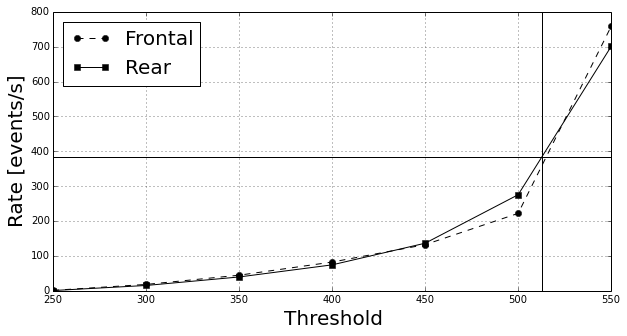
\includegraphics[scale=0.38]{Figures/Panel_cal.png}
   % \caption{Detection rate for the frontal and rear panel ranging discrimination thresholds from 250 UDAC to 550 UDAC. The red cross indicates the discrimination value for a 384 events/s expected rate at 990 m.a.s.l. }
    %\label{PanelRate}
%\end{figure}

%Afterward, the hodoscope was placed inside a laboratory under a 30 cm concrete shielding for performing the calibration using cosmic muons. The threshold value was set taking into account the expected muon rate in an area of 14400 cm$^²$ at  990 m.a.s.l ($\sim$ 1.6 muon/cm$^²$min). Fig. \ref{PanelRate} shows the detection rate for the frontal and rear panel depending of the discrimination threshold value (V$_{th0}$). The  expected rate is about 384 events/s which means a threshold of 510 DAC units.

%Otherwise, the number of photons reaching the  \textsl{SiPM} depends on the interaction point, the higher the distance between the  \textsl{SiPM} and the interaction point, the higher the attenuation in the photon yield. After analyzing 15 hours of data recording with the hodoscope pointing to 0 degrees zenith, it was found that the scintillator panel is less sensitive in average up to 40 $\%$ in the furthest corner from the  \textsl{SiPM} placement as in Fig. \ref{PanelData}.

%\begin{figure}[h]
 %   \centering
  %  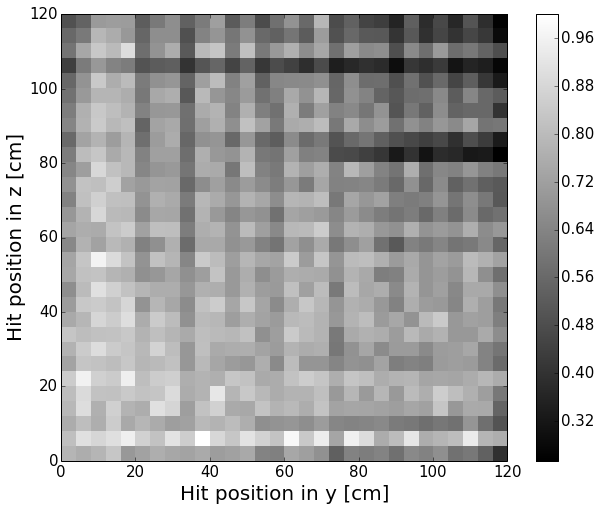
\includegraphics[scale=0.38]{Figures/PanelData.png}
   % \caption{Normalized hit histogram for the frontal panel with 15 hours of data. The locations of the \textsl{SiPMs} are in the bottom-left corner (0,0). In the furthest corner (120cm, 120cm) the detection rate decrease down to 30$\%$. }
    %\label{PanelData}
%\end{figure}

%%%%%%%%%%%%%%%%%%%%%%%%%%%
%%%%%%% SUBSECTION %%%%%%%%
%%%%%%%%%%%%%%%%%%%%%%%%%%%
\subsection{First WCD measurements}
\label{sec:wcd-data}%Jesus
% Voy por aquí
The \textsl{WCD} acquisition system records two signals from the \textsl{PMT}, anode, and the last dynode amplified 20 times to increase the measuring range with a 10 bits analog-to-digital converter digitizing both channels.

The digitized electric charge $Q_{ADC}$ recorded by the \textsl{WCD} electronics is defined,
\begin{equation}
\label{n_FE}
Q_{ADC} =  \frac{1}{RG_{a}}\sum_{i=0}^{N-1} V_{ADC} \Delta_T
\end{equation}
where $V_{ADC}$ is the digitized voltage, $\Delta_T$ is the time sampling step, $G_a$ is the amplification factor of the electronics front-end, $R$ is the sensitive resistance and $N$ es the number of samples. 

Then the number of detected \textsl{pe} is,
\begin{equation}
\label{n_FE}
N_{pe} = \frac{Q_{ADC}}{eG_{PMT}}
\end{equation}
where $G_{PMT}$ is the \textsl{PMT} gain and $e$ is the electron charge.

In this case, the \textsl{PMT} was biased with $1$kV reaching a $G_{PMT}\sim$0.3$\times10^6$. The conditioning electronics has an amplification factor $G_a = 20$ and $R = 50 \Omega$. The signal is digitized with a sampling frequency of $40$MHz ($\Delta_T$ = 25ns) and stored in a vector of $N$ = 12.  

